\section*{I.1.1.1}
Given
\[
	a = \begin{pmatrix} 1\\2\\2 \end{pmatrix}
	b = \begin{pmatrix} 3\\2\\1 \end{pmatrix}
\]
Then $a^Tb = 9$

\section*{I.1.1.2}
The \textit{l2-norm} or \textit{Euclidean norm} $||a|| = \sqrt{1^2 + 2^2 + 2^2} = 3$

\section*{I.1.1.3}
The outer product
\[
	ab^T = \begin{bmatrix}
		3 & 2 & 1 \\
		6 & 4 & 2 \\
		6 & 4 & 2
	       \end{bmatrix}
\]

\section*{I.1.1.4}
The inverse matrix of $M$ is
\[
	M^{-1} = \begin{bmatrix}
		1 & 0 & 0 \\
		0 & 0.25 & 0 \\
		0 & 0 & 0.5
	\end{bmatrix}
\]

\section*{I.1.1.5}
The matrix-vector product $Ma = \begin{pmatrix}1 \\ 8 \\ 4\end{pmatrix}$

\section*{I.1.1.6}
\[
	A = ab^T = \begin{bmatrix}
		3 & 6 & 6 \\
		2 & 4 & 4 \\
		1 & 2 & 2
	\end{bmatrix}
\]

\section*{I.1.1.7}
The rank of $A = 1$, because the rows are linearly dependent. We can verify this by observing
that the third row can produce the first and second rows with a multiple, e.g. the first row (3 6 6)
is the same as the third row (1 2 2) x 3.

\section*{I.1.1.8}
As $A$ is not full rank, it is not invertible.

\section*{I.1.2.1}
The derivative of $f(w) = (wx + b)^2$ with respect to $w$ is
\[
	(wx+b)^2 = w^2 x^2 + 2wxb+b^2 = \\
	2x^2w + 2xb = \\
	2x(xw + b)
\]

\section*{I.1.2.2}
In general
\[
	\left ( \frac{f}{g} \right )' (x) = \frac{f'(x) \cdot g(x) - f(x) \cdot g'(x)}{(g(x))^2}
\]

Therefore, differentiating for w we get:
\begin{align*}
	f(x) &= 1 \\
	f'(x) &= 0 \\
	g(x) &= (wx+b)^2 \\
	g'(x) &= 2x(wx+b) \\
	\left ( \frac{f}{g} \right )' (w) &= \frac{0 \cdot (wx+b)^2 - 1 \cdot 2x(wx+b)}{((wx+b)^2)^2} \\
	&= \frac{-1 \cdot 2x(wx+b)}{(wx+b)^4} \\
	&= \frac{-2x}{(wx+b)^3}
\end{align*}

\section*{I.1.2.3}
In general
\[
	\left ( f \cdot g \right )' (x) = f'(x) \cdot g(x) + f(x) \cdot g'(x)
\]

Therefore, differentiating for x we get:
\begin{align*}
	f(x) &= x \\
	g(x) &= e^x \\
	\left ( f \cdot g \right )' (x) &= 1e^x + xe^x
\end{align*}

\pagebreak
\section*{I.2.1}
The plots with gaussian distributions for (sigma, mu) pairs (-1,1), (0,2) and (2,3) can be
seen in Figure~\ref{fig:I.2.1}. The code for generating the plots can be found in \texttt{unigauss\_run.m}, 
and the code for our gaussian distribution function can be found in \texttt{unigauss.m}.

\begin{figure}[h!]
	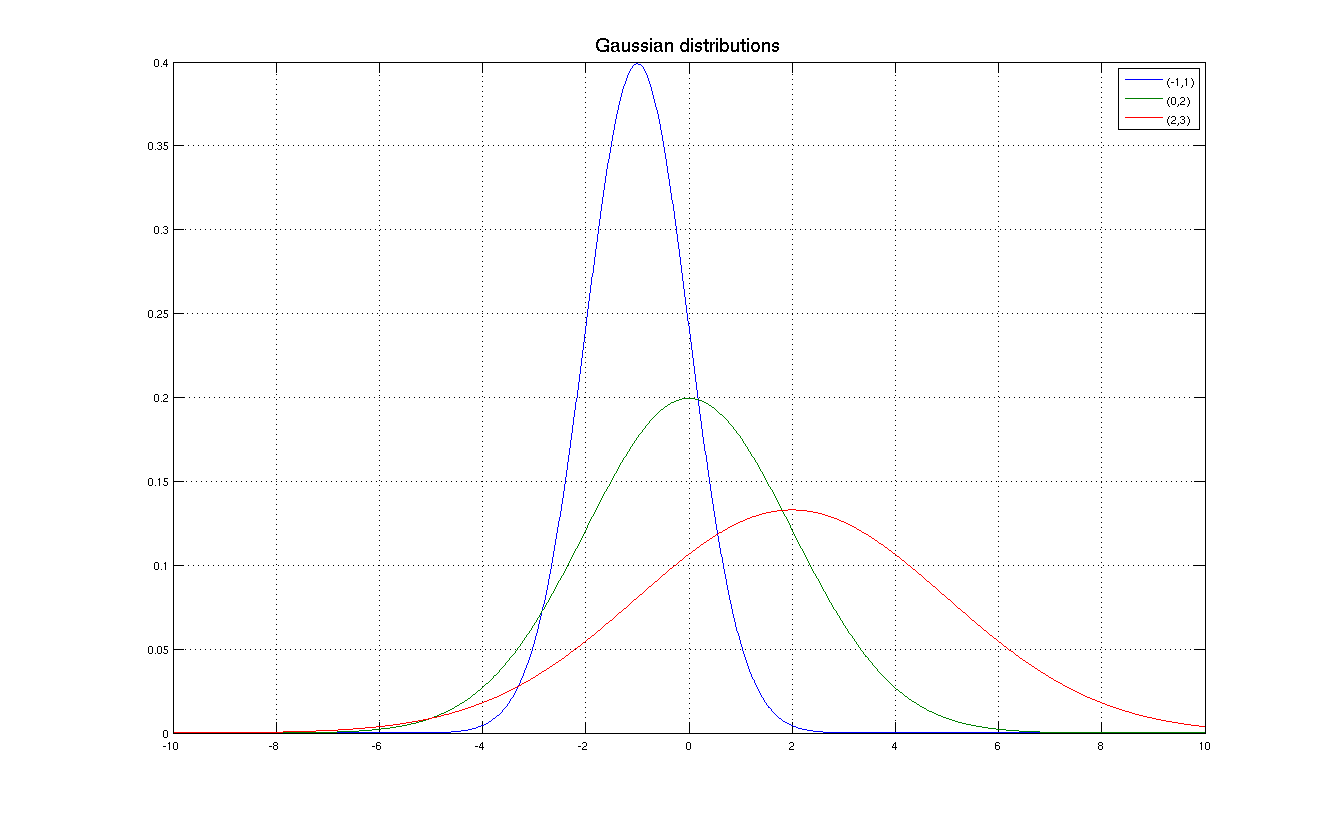
\includegraphics[width=0.5\textwidth]{img/unigauss}
	\caption{Gaussian distributions plotted with different values for (sigma, mu). \label{fig:I.2.1}}
\end{figure}

\section*{I.2.2}
Source code is available in \texttt{multigauss.m} and \texttt{multigauss\_run.m}.
\begin{figure}[h!]
	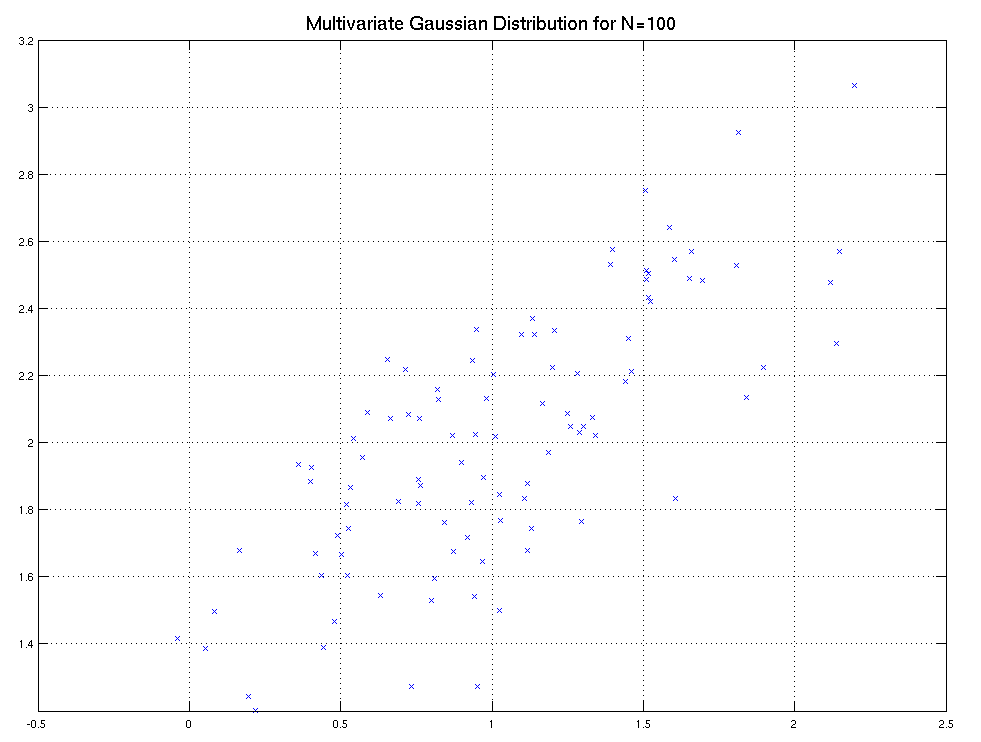
\includegraphics[width=0.5\textwidth]{img/multigauss}
	\caption{100 points drawn from a 2-dimensional Multivariate gaussian distribution. \label{fig:I.2.2}}
\end{figure}

\section*{I.2.3}
The l2 norm of $x$ is 
\begin{align*}
	mean  &= \begin{pmatrix}1 & 2\end{pmatrix}^T \\
	\mu   &= \begin{pmatrix}1.0006 & 1.9834\end{pmatrix}^T \\
	||x|| &= l2(mean - \mu) = 0.0366
\end{align*}
where $l2()$ is a function that calculates the \textit{Euclidean norm} or l2 norm of the vector $mean - \mu$.

Figure~\ref{fig:I.2.3} plots the points drawn along with a red circle for the calculated mean and a green circle
for $\mu$. There is a difference between the two because the mean is calculated based on the generated data drawn
from the multivariate gaussian distribution at random. If we had a number of points approaching infinite, the difference
would approach 0.

\begin{figure}[h!]
	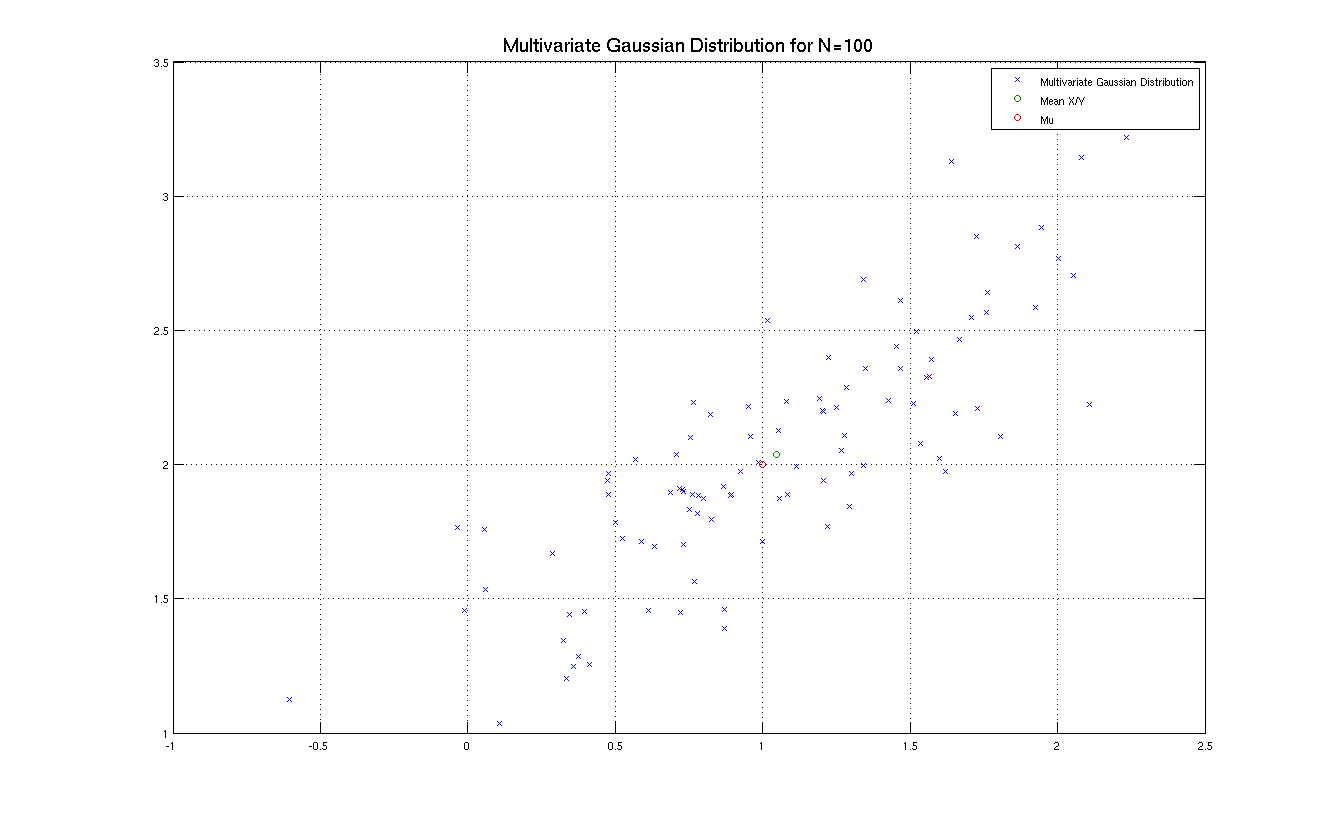
\includegraphics[width=0.5\textwidth]{img/multigaussmeanxy}
	\caption{100 points drawn from a 2-dimensional Multivariate gaussian distribution, plotted with
	the mean of the distribution and the value of $\mu$. \label{fig:I.2.3}}
\end{figure}

\FloatBarrier
\section*{I.2.4}
The covariance matrix is full rank 2 and thus has two eigenvectors and eigenvalues. Each eigenvector represents
a principal component (or linearly uncorrelated variable), and each eigenvalue a scalar representing the variance.
Intuitively, the eigenvectors form a scaled and translated coordinate system centered at the mean of the multivariate
Gaussian distribution ($\mu$). If an eigenvalue is 0, the dimensionality is reduced by one. The larger of the two
eigenvector/value pairs represents the direction where the ellipsis is widest.

\begin{figure}[h!]
	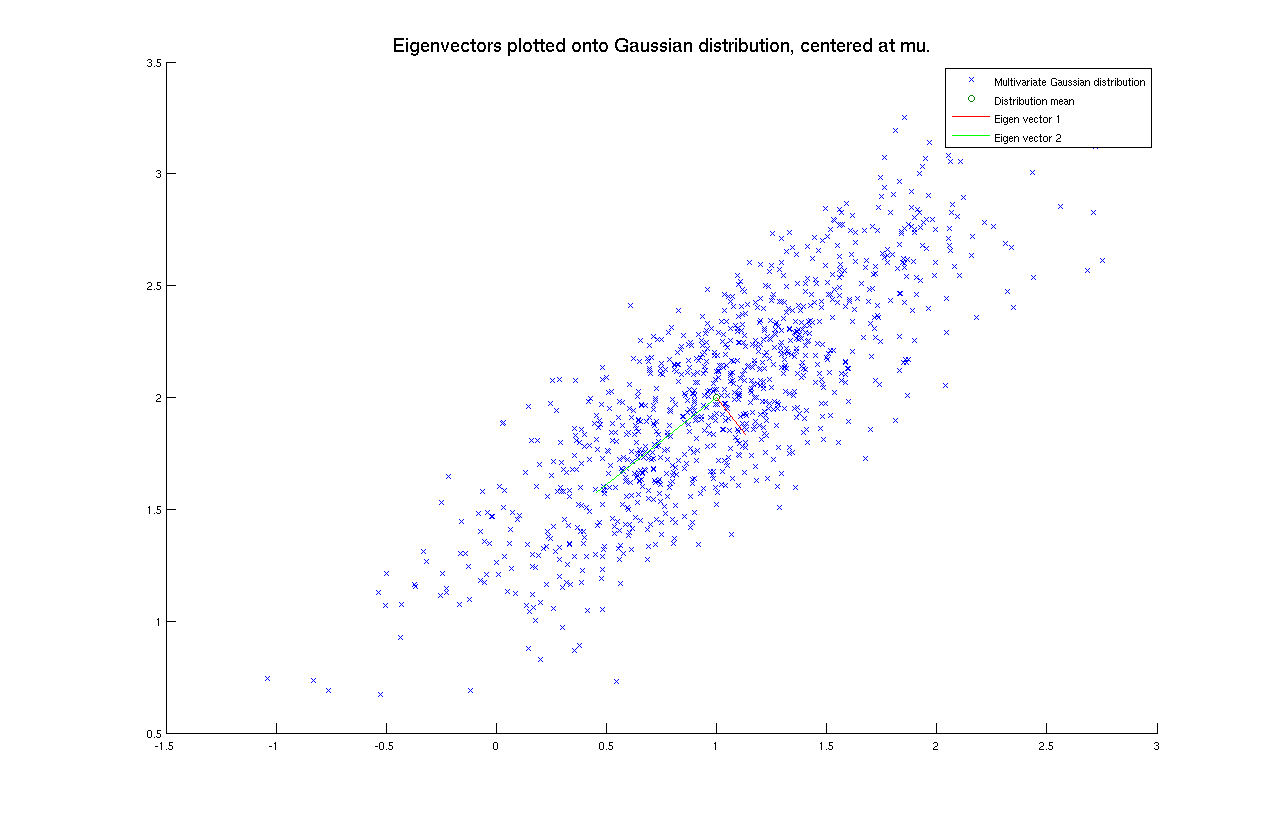
\includegraphics[width=0.5\textwidth]{img/multigausseigen}
	\caption{1000 points drawn from a 2-dimensional Multivariate gaussian distribution, plotted with the
	mean of the distribution, the value of $\mu$ and the two eigenvectors centered in the distribution $\mu$. \label{fig:I.2.4.1}}
\end{figure}


